\chapter{IMPLEMENTATION DETAILS}

The implementation of the system to convert hand-drawn circuit diagrams into simulation-ready netlists and digital schematics follows a modular approach, aligning with the pipeline described in the architecture and methodology.

\section{Dataset Manipulation and Preprocessing}

\subsection{Conversion of Annotation Formats}

To accommodate the multiple models in the pipeline (YOLOv7 for component detection and \gls{ocr} for value extraction), annotation files provided in the \gls{cghd} dataset in Pascal VOC (XML) format were converted into compatible formats. Likewise, for EasyOCR-inspired custom-trained \gls{ocr}, all text-sections needed to be cropped out from the image with corresponding labels (ground truth) and then fed to the fine-tuned model.

In Pascal VOC format, the information regarding the circuit and its components are stored in the following format as shown by the example below:

\begin{lstlisting}[language=XML, frame=none, numbers=none, backgroundcolor=, basicstyle=\ttfamily\fontsize{12}{14}\selectfont, label={lst:pascal-voc-example}]
<annotation>
    <folder>images</folder>
    <filename>C1_D1_P2.jpg</filename>
    <path>./drafter_1/images/C1_D1_P2.jpg</path>
    <source>
        <database>CGHD</database>
    </source>
    <size>
        <width>3024</width>
        <height>4032</height>
        <depth>3</depth>
    </size>
    <segmented>0</segmented>
    <object>
        <name>voltage.dc</name>
        <pose>Unspecified</pose>
        <truncated>0</truncated>
        <difficult>0</difficult>
        <bndbox>
            <xmin>327</xmin>
            <ymin>546</ymin>
            <xmax>604</xmax>
            <ymax>838</ymax>
            <rotation>10</rotation>
        </bndbox>
    </object>
</annotation>
\end{lstlisting}

For \gls{yolo}-based detection, XML annotations were converted to \gls{yolo} format (\texttt{.txt}) using a custom Python script. Each \texttt{.txt} file contains the class index and normalized bounding box coordinates in the format:

\begin{center}
\texttt{<class\_id> <x\_center> <y\_center> <width> <height>}
\end{center}

The pseudocode for the VOC to YOLO annotation conversion is as follows:

\begin{algorithm}
\caption{VOC to YOLO Annotation Conversion}
\label{algo:voc-to-yolo}
\begin{algorithmic}
\Require XML annotation file $X$, class map $C$, image width $W$, image height $H$
\Ensure List of YOLO formatted annotation lines $Y$
\State Parse XML file $X$ into tree structure
\State $Y \leftarrow \emptyset$
\For{all object nodes $o$ in XML root}
    \State $\text{clsname} \leftarrow$ class name of $o$
    \If{$\text{clsname} \notin C$}
        \State \textbf{continue}
    \EndIf
    \State $\text{clsid} \leftarrow C[\text{clsname}]$
    \State Extract bounding box $(x_{\min}, y_{\min}, x_{\max}, y_{\max})$ from $o$
    \State Convert VOC coordinates to normalized YOLO format
    \State $x_{\text{center}} \leftarrow \frac{x_{\min} + x_{\max}}{2W}$
    \State $y_{\text{center}} \leftarrow \frac{y_{\min} + y_{\max}}{2H}$
    \State $w \leftarrow \frac{x_{\max} - x_{\min}}{W}$
    \State $h \leftarrow \frac{y_{\max} - y_{\min}}{H}$
    \State Append formatted string $(x_{\text{center}}, y_{\text{center}}, w, h)$ to $Y$
\EndFor
\State \Return $Y$
\end{algorithmic}
\end{algorithm}

The calculations run for this conversion is as follows:

\begin{equation}
x_{\text{center}} = \frac{327 + 604}{2 \times 3024} = \frac{465.5}{3024} = 0.1539
\label{eq:voc-yolo-x}
\end{equation}

\begin{equation}
y_{\text{center}} = \frac{546 + 838}{2 \times 4032} = \frac{692}{4032} = 0.1716
\label{eq:voc-yolo-y}
\end{equation}

\begin{equation}
w = \frac{604 - 327}{3024} = \frac{277}{3024} = 0.0916
\label{eq:voc-yolo-w}
\end{equation}

\begin{equation}
h = \frac{838 - 546}{4032} = \frac{292}{4032} = 0.0724
\label{eq:voc-yolo-h}
\end{equation}

This gives the information required by \gls{yolo} in the appropriate format. It is convention to save this new annotation file in the same directory as the image.

Likewise, for \gls{ocr} compatibility, the same Pascal VOC annotations were converted to \gls{lmdb} format. \gls{lmdb} is a high-speed key-value store where each key corresponds to an index and each value contains an image-text pair (serialized).

The pseudocode for the conversion of Pascal VOC format to \gls{ocr}-compatible \gls{lmdb} file format is as follows:

\begin{algorithm}
\caption{Image Cropping and LMDB Dataset Creation}
\label{algo:image-crop-lmdb}
\begin{algorithmic}
\Require Input image file $I$, crop coordinates $(y_{\min}, y_{\max}, x_{\min}, x_{\max})$, target size $(W, H)$
\Ensure \gls{lmdb} database containing image-label pairs
\State Load image $I$ into memory
\State Crop image using coordinates $[y_{\min} : y_{\max}, x_{\min} : x_{\max}]$
\State Resize cropped image to size $(W, H)$
\State Convert cropped image to byte representation
\State Convert image array to PIL image
\State Initialize in-memory byte buffer
\State Save image to buffer in JPEG format
\State Extract byte stream from buffer
\State Store image and label in \gls{lmdb}
\State Open \gls{lmdb} environment with predefined map size
\State Begin write transaction
\State Store image bytes with key \texttt{image-00001}
\State Store corresponding label with key \texttt{label-00001}
\State Store total sample count with key \texttt{num-samples}
\State Commit transaction
\State \Return \gls{lmdb} environment
\end{algorithmic}
\end{algorithm}

After this script is run in its entirety, a file in \gls{lmdb} format, as is expected by \gls{ocr}, is received as shown in the example below:

\begin{lstlisting}[frame=none, numbers=none, backgroundcolor=, basicstyle=\ttfamily\fontsize{12}{14}\selectfont, label={lst:lmdb-example}]
Key: b'image-00001'
Value: b'\xff\xd8\xff\xe0\x00\x10JFIF...'

Key: b'label-00001'
Value: b'voltage.dc'

Key: b'num-samples'
Value: b'000001'
\end{lstlisting}

After necessary conversion, the dataset was ready for being plugged into the required models for fine-tuning them. But first, some experimentation was done with different forms of image augmentation techniques.

\subsection{Image Augmentation}

Since the dataset contains handwritten circuit diagrams captured under variable lighting and orientations, several augmentation techniques were applied to improve model generalization including Contrast Enhancement (global) and Adaptive Brightness Adjustment by factors of 0.8 and 1.2. Furthermore, geometric augmentation techniques, like spatial flipping (both horizontally and vertically) and rotation (e.g., $90^\circ$ or random rotation) proved to be unwise operations for this project. For example, if a ``C'' is rotated by $90^\circ$, the ``C'' now resembles a ``U'', and the same applies to flipping (``M'' might look like ``W'', for example). Rather than increasing accuracy, it was realized that using rotation or flipping would simply confuse the model. 

\subsection{Fine-tuning YOLOv5 and YOLOv7 for Component Detection}

YOLOv5 was initially used for benchmarking, and later upgraded to YOLOv7 for better accuracy and inference speed (comparison shown in the Results section). Training and fine-tuning were done using the \gls{cghd} dataset after converting into \gls{yolo}-compatible format.

The training parameters employed are as follows:

\begin{itemize}
    \item \textbf{Number of classes:} 61
    \item \textbf{Training split:} 70\% training, 10\% validation, 20\% testing
    \item \textbf{Epochs:} 200 (for YOLOv5), 100 (for YOLOv7)
    \item \textbf{Image size:} $416 \times 416$ pixels
    \item \textbf{Batch size:} 16 (for YOLOv5), 32 (for YOLOv7)
    \item \textbf{Optimizer:} \gls{sgd} (Stochastic Gradient Descent)
    \item \textbf{Learning rate:} 0.01 (initial)
    \item \textbf{Augmentations used in training:} Mosaic Augmentation, \gls{hsv} Augmentation, Random rotating/flipping
\end{itemize}


\subsection{Class Consolidation and Retraining}

Satisfactory results were not obtained through the initial 61-class approach. To improve the performance, consolidation of 61 classes into 15 was done, and the models were retrained on this new taxonomy. 

\begin{table}[H]
\centering
\caption{Consolidation of Original Classes into Unified YOLO Classes}
\label{tab:class_consolidation}
\begin{tabular}{@{}clp{8.2cm}@{}}
\toprule
\textbf{Class Code} & \textbf{Class Name} & \textbf{Consolidated Classes} \\
\midrule
0  & capacitor & capacitor.adjustable, capacitor.polarized, capacitor.unpolarized \\
1  & crossover & crossover \\
2  & diode & diode, diode.light\_emitting, diode.thyrector, diode.zener \\
3  & gnd & gnd \\
4  & inductor & inductor, inductor.coupled, inductor.ferrite \\
5  & integrated\_circuit & integrated\_circuit, integrated\_circuit.ne555, integrated\_circuit.voltage\_regulator \\
6  & junction & junction \\
7  & operational\_amplifier & operational\_amplifier, operational\_amplifier.schmitt\_trigger \\
8  & resistor & resistor, resistor.adjustable, resistor.photo \\
9  & switch & switch \\
10 & terminal & terminal \\
11 & text & text \\
12 & transistor & transistor.bjt, transistor.fet, transistor.photo \\
13 & voltage & voltage.ac, voltage.battery, voltage.dc \\
14 & vss & vss \\
\bottomrule
\end{tabular}
\end{table}

A merge mapping was applied to the original annotations, grouping visually similar subclasses (e.g., capacitor.polarized and capacitor.unpolarized into capacitor) as shown in the Table \ref{tab:class_consolidation}. This consolidation is done not only considering visual similarity but also based on the usage i.e, the resulting 15 classes make up the majority of basic-level circuits Four \gls{yolo} architectures were then trained on this 15-class dataset for benchmarking:

\begin{itemize}
    \item \textbf{YOLOv7 (retrained):} 100 epochs, batch size 16, image size $640 \times 640$
    \item \textbf{YOLOv8:} 100 epochs, batch size 16, image size $640 \times 640$
    \item \textbf{YOLOv11:} 100 epochs, batch size 16, image size $640 \times 640$
    \item \textbf{YOLOv26:} 100 epochs, batch size 16, image size $640 \times 640$
\end{itemize}

All models were trained on identical data splits with the same augmentation pipeline, confidence threshold of 0.25, and \gls{iou} threshold of 0.45. 

\subsection{Implementation of Custom Text Recognition (OCR)}

To extract textual information such as resistor values, capacitor labels, and other component annotations from the circuit diagrams, a \gls{crnn}-based custom \gls{ocr} model was trained, and implemented. The input image in cropped form (cropped for each text component) was passed through this model after training, which returned the content of each detected text element. The position of said text element was found using bounding boxes from YOLOv7. This allowed us to localize and read numerical values or labels directly from the circuit.

Three different modules, each for feature extraction, sequence modeling, and prediction were trained based on the DTRB framework. Initially, simply EasyOCR was also attempted; however, this didn't yield usable results, ultimately requiring training from scratch. The training, which was done for 27 epochs, had early stopping as it's accuracy per epoch failed to achieve even a 0.01\% increase within 5 epochs. Other training details include:

\begin{itemize}
    \item \textbf{Training epochs:} 27 (with early stopping)
    \item \textbf{Image Height:} 64px (fixed for all croppings)
    \item \textbf{Aspect Ratio:} 4:1 (allowing for variable width)
    \item \textbf{Learning Rate:} 0.01 (initial)
\end{itemize}

\subsection{Fine-tuning TrOCR for Text Recognition}

Following the initial custom \gls{crnn} approach, a second \gls{ocr} model was implemented using Microsoft's TrOCR-small-printed architecture. Unlike the \gls{crnn} model which was trained from scratch, TrOCR was fine-tuned from pre-trained weights, leveraging transfer learning from large-scale printed text datasets.

The fine-tuning was performed on cleaned text crops extracted from the \gls{cghd} dataset. All text crops from a single image were processed in one forward pass, and per-token log-probability was averaged across the generated sequence with following details:

\begin{itemize}
    \item \textbf{Base model:} Microsoft TrOCR-small-printed (pre-trained)
    \item \textbf{Fine-tuning epochs:} 3
    \item \textbf{Checkpoint:} Epoch 2 (best validation performance)
    \item \textbf{Inference precision:} float16 (half-precision for GPU acceleration)
    \item \textbf{Maximum output tokens:} 16 (sufficient for values like ``10k$\Omega$'', ``100$\mu$F'')
\end{itemize}

The TrOCR model is integrated into the pipeline through a singleton service that lazy-loads the processor and model weights when it is first invoked.

\subsection{Line Detection Algorithm Implementation}

Any sort of line detection algorithm in service of detecting wires in a circuit diagram exploit the regularity inherent to standard circuit diagrams. This junction-based method takes the junction points that YOLOv7 has already picked up and treats them as anchor nodes for rebuilding the wiring layout through geometry.

\begin{algorithm}
\caption{Wire Classification and Alignment}
\label{algo:wire-classification-impl}
\begin{algorithmic}
\Require Set of junctions $J$, angular tolerance $\omega_{\text{tol}} = 18^\circ$, grid size $g = 16$
\Ensure Set of raw wire segments $S$
\State $S \leftarrow \emptyset$
\For{all pairs $(j_a, j_b) \in \text{Combinations}(J, 2)$}
    \State $\Delta x \leftarrow j_b.x - j_a.x$
    \State $\Delta y \leftarrow j_b.y - j_a.y$
    \State $\theta \leftarrow \text{atan2}(\Delta y, \Delta x)$
    \If{$|\theta| \le \omega_{\text{tol}} \lor |\theta - 180^\circ| \le \omega_{\text{tol}}$}
        \State \textbf{Horizontal alignment check}
        \State $y_{\text{avg}} \leftarrow \frac{j_a.y + j_b.y}{2}$
        \State $y_{\text{snap}} \leftarrow \text{Round}\left(\frac{y_{\text{avg}}}{g}\right) \times g$
        \State $S \leftarrow S \cup \{(H, y_{\text{snap}}, \min(j_a.x, j_b.x), \max(j_a.x, j_b.x))\}$
    \ElsIf{$|\theta - 90^\circ| \le \omega_{\text{tol}} \lor |\theta - 270^\circ| \le \omega_{\text{tol}}$}
        \State \textbf{Vertical alignment check}
        \State $x_{\text{avg}} \leftarrow \frac{j_a.x + j_b.x}{2}$
        \State $x_{\text{snap}} \leftarrow \text{Round}\left(\frac{x_{\text{avg}}}{g}\right) \times g$
        \State $S \leftarrow S \cup \{(V, x_{\text{snap}}, \min(j_a.y, j_b.y), \max(j_a.y, j_b.y))\}$
    \EndIf
\EndFor
\State \Return $S$
\end{algorithmic}
\end{algorithm}

Pairwise comparison has a predictable side effect: redundant overlapping segments pile up for the same wire. Multiple separate segments are seen for multiple junctions if they are sitting on the same line, but in reality, there exists only one continuous wire. To address this, collinear segment merging is needed.

After classifying the segments as horizontal or vertical, the overlapping or neighboring line segments get merged together. During each merge, the axis coordinate of whichever segment is longer takes priority, since a longer stroke is a more trustworthy indicator of where the wire actually runs.

\begin{algorithm}
\caption{Collinear Segment Merging}
\label{algo:segment-merging-impl}
\begin{algorithmic}
\Require List of segments $L$, gap tolerance $\omega$
\Ensure List of merged segments $M$
\State Sort $L$ by primary axis, then by starting coordinate
\State $M \leftarrow \emptyset$
\State $\text{curr} \leftarrow L[0]$
\For{all $\text{next} \in L[1 \ldots N]$}
    \If{$|\text{curr.axis} - \text{next.axis}| \le \omega \land \text{next.start} \le \text{curr.end} + \omega$}
        \State $\text{curr.start} \leftarrow \min(\text{curr.start}, \text{next.start})$
        \State $\text{curr.end} \leftarrow \max(\text{curr.end}, \text{next.end})$
        \If{$\text{Length}(\text{next}) > \text{Length}(\text{curr})$}
            \State \textbf{Preserve axis of the longer segment}
            \State $\text{curr.axis} \leftarrow \text{next.axis}$
        \EndIf
    \Else
        \State $M \leftarrow M \cup \{\text{curr}\}$
        \State $\text{curr} \leftarrow \text{next}$
    \EndIf
\EndFor
\State $M \leftarrow M \cup \{\text{curr}\}$
\State \Return $M$
\end{algorithmic}
\end{algorithm}

The wire–component intersection detection algorithm pinpoints where detected wire segments meet component bounding boxes. YOLOv7 annotations supply the component regions, which then get translated into pixel coordinates. Every horizontal or vertical wire is checked against each component box's edges for geometric intersection. Those intersection points pin down how the circuit is actually wired together, and the frontend can optionally render them for visual verification.

\begin{algorithm}
\caption{Wire-Component Intersection Detection}
\label{algo:wire-component-intersection-impl}
\begin{algorithmic}
\Require Wire segments $W$, \gls{yolo} label file $L$, image width $I_w$, image height $I_h$
\Ensure Set of intersection points $P$
\State Parse label file $L$
\State Convert normalized bounding boxes to pixel coordinates
\State Discard non-component classes
\State Store component boxes $B$
\State \textbf{Detect intersections between wires and components}
\State $P \leftarrow \emptyset$
\For{all wire $w \in W$}
    \For{all box $b \in B$}
        \If{$w$ is horizontal and crosses left or right edge of $b$}
            \State Add intersection point to $P$
        \ElsIf{$w$ is vertical and crosses top or bottom edge of $b$}
            \State Add intersection point to $P$
        \EndIf
    \EndFor
\EndFor
\State Draw wires, component boxes, and intersection points on image
\State Save output visualization
\State \Return $P$
\end{algorithmic}
\end{algorithm}

\section{Line Detection via Path Finding}

The algorithm behind the path-finding line detection pipeline first splits the work into a handful of stages. First, a spatial map of node regions is assembled. Multi-head BFS traversal then crawls through skeleton pixels to uncover which nodes connect to which. Spurious self-edges get pruned in a final cleanup pass.

Building a node identification map kicks off the whole process. This map contains information regarding if a particular pixel falls inside a node (node's circuilar disk region) or not. Algorithm~\ref{alg:node_id_map} details the construction of this node id map.

\begin{algorithm}[H]
\caption{Build Node ID Map}
\label{alg:node_id_map}
\begin{algorithmic}[1]
\Require Skeleton image $S$ of size $H \times W$, list of nodes $\mathcal{N} = \{(x_0, y_0), \ldots, (x_{n-1}, y_{n-1})\}$, radius $r$
\Ensure Node ID map $M$ of size $H \times W$

\State $M \gets$ array of size $H \times W$ initialized to $-1$
\State $\mathcal{D} \gets \text{DiskMask}(r)$

\For{$i \gets 0$ \textbf{to} $n-1$}
    \State $(n_x, n_y) \gets \mathcal{N}[i]$
    \For{each $(dy, dx) \in \mathcal{D}$}
        \State $(p_y, p_x) \gets (n_y + dy, n_x + dx)$
        \If{$0 \leq p_y < H$ \textbf{and} $0 \leq p_x < W$}
            \State $M[p_y][p_x] \gets i$
        \EndIf
    \EndFor
\EndFor

\State \Return $M$
\end{algorithmic}
\end{algorithm}

Once the node ID map is constructed, the algorithm performs a breadth-first search from each node to discover its neighbors along the skeleton. The BFS starts from the boundary of each node's disk region and traverses skeleton pixels using 8-connectivity. When this BFS traversal meets a pixel belonging to a different node, that node is recorded as a neighbor which terminates the branch. This ensures that each skeleton path is followed until it reaches another endpoint. Algorithm~\ref{alg:bfs_node} describes this procedure.

\begin{algorithm}[H]
\caption{BFS Neighbors for Node}
\label{alg:bfs_node}
\begin{algorithmic}[1]
\Require Node index $i$, nodes $\mathcal{N}$, skeleton $S$, node ID map $M$, radius $r$
\Ensure Set of neighbor node indices $\mathcal{A}_i$

\State $(n_x, n_y) \gets \mathcal{N}[i]$
\State $\mathcal{A}_i \gets \emptyset$
\State $V \gets$ boolean array of size $H \times W$ initialized to \texttt{false}
\State $\mathcal{D} \gets \text{DiskMask}(r)$

\For{each $(dy, dx) \in \mathcal{D}$}
    \State $(p_y, p_x) \gets (n_y + dy, n_x + dx)$
    \If{$0 \leq p_y < H$ \textbf{and} $0 \leq p_x < W$}
        \State $V[p_y][p_x] \gets \texttt{true}$
    \EndIf
\EndFor

\State $Q \gets$ empty queue
\For{each $(dy, dx) \in \mathcal{D}$}
    \State $(p_y, p_x) \gets (n_y + dy, n_x + dx)$
    \For{each $(n_y', n_x') \in \text{Neighbors8}(p_y, p_x)$}
        \If{$\neg V[n_y'][n_x']$ \textbf{and} $S[n_y'][n_x'] > 0$}
            \State $V[n_y'][n_x'] \gets \texttt{true}$
            \State $Q.\text{enqueue}((n_y', n_x'))$
        \EndIf
    \EndFor
\EndFor

\While{$Q$ is not empty}
    \State $(c_y, c_x) \gets Q.\text{dequeue}()$
    \State $j \gets M[c_y][c_x]$
    
    \If{$j \neq -1$ \textbf{and} $j \neq i$}
        \State $\mathcal{A}_i \gets \mathcal{A}_i \cup \{j\}$
        \State \textbf{continue}
    \EndIf
    
    \For{each $(n_y', n_x') \in \text{Neighbors8}(c_y, c_x)$}
        \If{$\neg V[n_y'][n_x']$ \textbf{and} $S[n_y'][n_x'] > 0$}
            \State $V[n_y'][n_x'] \gets \texttt{true}$
            \State $Q.\text{enqueue}((n_y', n_x'))$
        \EndIf
    \EndFor
\EndWhile

\State \Return $\mathcal{A}_i$
\end{algorithmic}
\end{algorithm}

The final step removes spurious connections between endpoints that belong to the same detected object. Since line segment bounding boxes produce two endpoints each, the BFS may incorrectly connect these as neighbors via the skeleton segment within the bounding box. By maintaining a list of endpoint pairs from the same object, these self-edges are explicitly removed from the adjacency graph. Algorithm~\ref{alg:remove_self} implements this filtering.

\begin{algorithm}[H]
\caption{Remove Self-Edges (Same-Object Connections)}
\label{alg:remove_self}
\begin{algorithmic}[1]
\Require Adjacency $\mathcal{G}$, endpoint pairs $\mathcal{P} = \{(p_1^{(k)}, p_2^{(k)})\}_{k=1}^{m}$, nodes $\mathcal{N}$
\Ensure Filtered adjacency $\mathcal{G}'$

\State $\mathcal{G}' \gets \mathcal{G}$

\For{each $(p_1, p_2) \in \mathcal{P}$}
    \State $i \gets \text{FindIndex}(p_1, \mathcal{N})$
    \State $j \gets \text{FindIndex}(p_2, \mathcal{N})$
    
    \If{$i \neq -1$ \textbf{and} $j \neq -1$}
        \State $\mathcal{G}'[i] \gets \mathcal{G}'[i] \setminus \{j\}$
        \State $\mathcal{G}'[j] \gets \mathcal{G}'[j] \setminus \{i\}$
    \EndIf
\EndFor

\State \Return $\mathcal{G}'$
\end{algorithmic}
\end{algorithm}

\subsection{Complexity of Implemented Algorithm}

This section analyzes the computational complexity of the line detection pipeline. Let $H, W$ denote the image dimensions, $n$ the number of nodes (endpoints), $r$ the disk radius for node regions, and $P$ the number of skeleton pixels (typically $P \ll H \times W$).

\begin{table}[H]
\centering
\caption{Time complexity breakdown for Multi-Head BFS algorithm}
\label{tab:time_complexity}
\begin{tabular}{@{}lll@{}}
\toprule
\textbf{Operation} & \textbf{Complexity} & \textbf{Description} \\
\midrule
Node ID Map Construction & $O(n \cdot r^2)$ & Each node marks $\pi r^2$ pixels \\
Single Node BFS & $O(P)$ & Each skeleton pixel visited at most once \\
Complete Adjacency Build & $O(n \cdot P)$ & BFS from each of $n$ nodes \\
Self-Edge Removal & $O(m)$ & $m$ = number of endpoint pairs \\
\midrule
\textbf{Total} & $O(n \cdot r^2 + n \cdot P)$ & Dominated by BFS traversals \\
\bottomrule
\end{tabular}
\end{table}

Table~\ref{tab:time_complexity} summarizes the time complexity of each operation in the pipeline.

\begin{table}[H]
\centering
\caption{Space complexity breakdown for Multi-Head BFS algorithm}
\label{tab:space_complexity}
\begin{tabular}{@{}lll@{}}
\toprule
\textbf{Data Structure} & \textbf{Space} & \textbf{Description} \\
\midrule
Skeleton Image $S$ & $O(H \times W)$ & Binary image storage \\
Node ID Map $M$ & $O(H \times W)$ & Integer array for node mapping \\
Visited Array $V$ & $O(H \times W)$ & Per-BFS boolean array \\
BFS Queue $Q$ & $O(P)$ & Maximum skeleton pixels in queue \\
Adjacency $\mathcal{G}$ & $O(n + E)$ & $E$ = number of edges \\
Disk Offsets $\mathcal{D}$ & $O(r^2)$ & Precomputed disk mask \\
\midrule
\textbf{Total} & $O(H \times W + n + E)$ & Dominated by image arrays \\
\bottomrule
\end{tabular}
\end{table}

Table~\ref{tab:space_complexity} details the memory requirements of the algorithm.


The visited array can be reused across BFS calls with a reset, or alternatively, a hash set can be used for sparse skeletons to reduce visited storage to $O(P)$.
For typical skeleton images where $P = O(H + W)$ (linear in image perimeter), the overall complexity is:
\[
T(n, H, W, r) = O(n \cdot r^2 + n \cdot (H + W)) = O(n \cdot (r^2 + H + W))
\]
In the real world, this approach can be considered efficient because it scales with the number of nodes, but it is bound by the physical resolution of the image sensor.

\subsection{Crossover Dissolution}

After the adjacency graph is constructed by Multi-Head BFS, crossover nodes must be resolved into their true topology. A crossover represents two wires crossing without connecting, and is initially represented as a single graph node with four neighbors. These crossover nodes are replaced by two direct connections, as described by Algorithm~\ref{algo:crossover-dissolution}.

\begin{algorithm}[H]
\caption{Crossover Dissolution Algorithm}
\label{algo:crossover-dissolution}
\begin{algorithmic}[1]
\Require Adjacency graph $\mathcal{G}$, node positions $\mathbf{p}$, detection results $\mathcal{R}$
\Ensure Modified graph $\mathcal{G}$ with crossovers dissolved

\For{each detection $r \in \mathcal{R}$ with $r.\mathrm{cls} = 1$}
    \State $a \gets$ node index of $r$'s endpoint in $\mathbf{p}$
    \If{$a = -1$ \textbf{or} $|\mathcal{G}[a]| \neq 4$}
        \State \textbf{continue}
    \EndIf
    \State $\{n_1, n_2, n_3, n_4\} \gets \mathcal{G}[a]$
    \For{each neighbor $n_k$}
        \State $\hat{\mathbf{d}}_k \gets \dfrac{\mathbf{p}[n_k] - \mathbf{p}[a]}{\|\mathbf{p}[n_k] - \mathbf{p}[a]\|}$
    \EndFor
    \State $S^* \gets +\infty$, \; $\Pi^* \gets \varnothing$
    \For{each pairing $\Pi = \{(n_i, n_j), (n_k, n_l)\}$ of the 4 neighbors into 2 pairs}
        \State $S \gets \hat{\mathbf{d}}_i \cdot \hat{\mathbf{d}}_j + \hat{\mathbf{d}}_k \cdot \hat{\mathbf{d}}_l$
        \If{$S < S^*$}
            \State $S^* \gets S$, \; $\Pi^* \gets \Pi$
        \EndIf
    \EndFor
    \State $\{(n_a, n_b), (n_c, n_d)\} \gets \Pi^*$
    \If{$\hat{\mathbf{d}}_a \cdot \hat{\mathbf{d}}_b > -0.7$ \textbf{or} $\hat{\mathbf{d}}_c \cdot \hat{\mathbf{d}}_d > -0.7$}
        \State \textbf{continue}
    \EndIf
    \For{each neighbor $n_k \in \{n_a, n_b, n_c, n_d\}$}
        \State $\mathcal{G}[n_k] \gets \mathcal{G}[n_k] \setminus \{a\}$
    \EndFor
    \State Remove $a$ from $\mathcal{G}$
    \State Add edges $(n_a, n_b)$ and $(n_c, n_d)$ to $\mathcal{G}$
\EndFor

\State \Return $\mathcal{G}$
\end{algorithmic}
\end{algorithm}

\section{Web App Implementation and Interaction}

The frontend was built using React.js and Next.js alongside CircuitJS. To bring all the frontend features to life, such as resizing, moving, rotating, renaming, etc. of the circuit elements with proper integration with the backend, additional packages and libraries like react-draggable and the KiCad Symbol Library were used. The backend of the CIRCUITRON system is a bunch of \gls{rest} \gls{api} endpoints that handle all the functions of the system such as uploading the circuit sketch, edit schematics (using temporary storage for changes), generate schematic, correction of values of components, etc.

\begin{figure}[H]
    \centering
    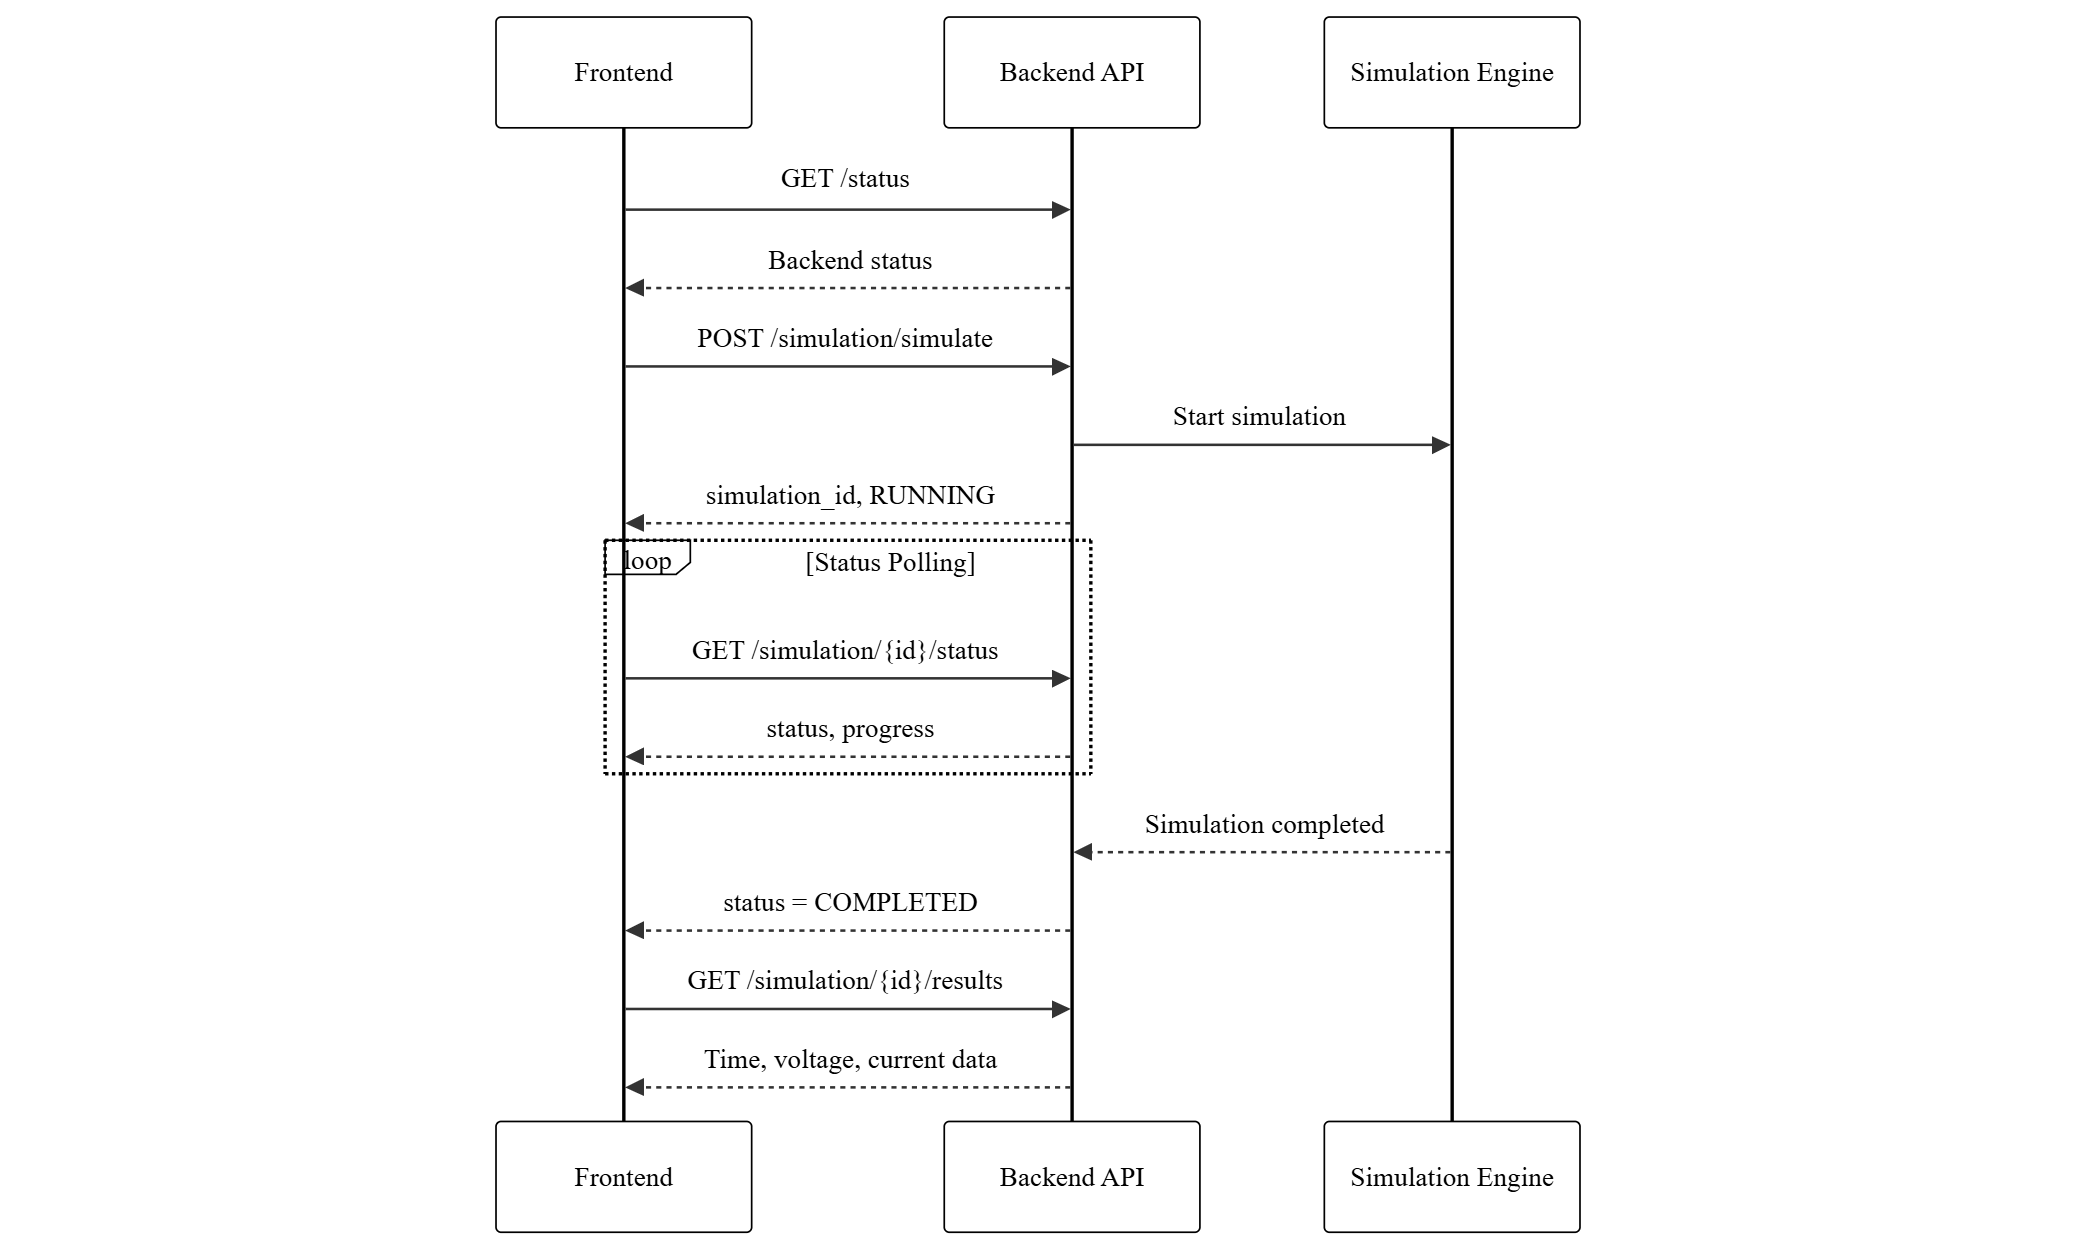
\includegraphics[width=\textwidth]{src/images/figures/backend_req_res.png}    \caption{Interaction Diagram for the Web Application}
    \label{fig:webapp-interaction}
\end{figure}

The endpoints defaults to JSON for communication and uses HTTP status codes for error reporting. The edits stored in temporary storage are made permanent through regular polling between backend and frontend (initiated by frontend). The simulation is handled, primarily, using an open source browser-based electronic circuit simulator named CircuitJS. Internally, CircuitJS mathematically models the circuit in the form of matrices, simplifying computations.

\section{Error Handling}

TTo handle errors in this project, foremost the errors in the output of the individual modules need to be controlled and only then can the accumulated error be kept in check. The performance metrics tabulated in the previous section are to be strictly adhered to if there's any hope of generating the CircuitJS compatible text file (and digital schematic) with nominal errors.

For the reduction of false matches and \gls{ocr} noise, post-processing techniques such as value format validation, confidence filtering, and text cleanup can be implemented. Value format validation ensures only strings that match known (and appropriate) electrical units, say $10k$, $1\mu F$, $5V$ are retained. Confidence filtering helps discard \gls{ocr} results with low confidence scores, and text cleanup normalizes ambiguous symbols such as converting ``O'' to ``0'', ``$\mu$'' to ``u''.

A basic pseudocode for sample value format validation is as follows:

\begin{algorithm}
\caption{Validation and Filtering of OCR Component Values}
\label{algo:ocr-validation}
\begin{algorithmic}
\Require OCR detected text entries $T$
\Ensure Filtered list of valid component values $V$
\State Define regular expression patterns for resistance, capacitance, and voltage
\State $V \leftarrow \emptyset$
\For{all text entry $t \in T$}
    \If{$t.\text{text}$ matches any defined pattern}
        \State Append $t$ to $V$
    \EndIf
\EndFor
\State \Return $V$
\end{algorithmic}
\end{algorithm}

The list of components shown here is in no way meant to be exhaustive; rather it is to show how this pseudocode ensures that only valid electrical component values are used in the final component-to-value mapping and schematic generation.

To prevent propagating error (error from the output of YOLOv7 bleeding into \gls{ocr}, for instance), a combined confidence threshold checking mechanism can be implemented which marks an item as uncertain if the confidence score from YOLOv7 is less than a certain value (e.g., 0.6) and the same from \gls{ocr} is less than a certain value (e.g., 0.85). For more robustness, a human-in-the-loop mechanism can be implemented which prompts the user to manually approve or correct \gls{ocr}-predicted values, fix connection errors, etc. This can be implemented to trigger when the confidence score is below the set threshold or when other error handling mechanisms such as value format validation fail. The pseudocode for this is as follows:

\begin{algorithm}
\caption{Confidence-Based Error Checking and Validation}
\label{algo:confidence-validation}
\begin{algorithmic}
\Require Module outputs $O$, confidence threshold $\omega$, format validation function $f$
\Ensure Valid outputs $V$ and uncertain outputs $U$
\State $V \leftarrow \emptyset$
\State $U \leftarrow \emptyset$
\For{all item $o \in O$}
    \If{$o.\text{confidence} \ge \omega \land f(o.\text{value})$}
        \State Append $o$ to $V$
    \Else
        \State Append $o$ to $U$
    \EndIf
\EndFor
\If{$U \ne \emptyset$}
    \State Trigger manual override
\EndIf
\State \Return $(V, U)$
\end{algorithmic}
\end{algorithm}
